% !TeX spellcheck = en_US
%*******************************************************************************
%****************************** Third Chapter *********************************
%*******************************************************************************
\chapter{Related Work}
\label{chapter3}
% **************************** Define Graphics Path **************************
\ifpdf
    \graphicspath{{Chapter3/Figs/Raster/}{Chapter3/Figs/PDF/}{Chapter3/Figs/}}
\else
    \graphicspath{{Chapter3/Figs/Vector/}{Chapter3/Figs/}}
\fi

This chapter presents different studies about how effective are social robots for the treatment of ASD children, which are the best design choices and which target behaviors can be reached using robots.  
\section{Social Robots and Children with ASD}
Computed-mediated therapy model have been developed, such as imaginative story telling\cite{howsmon2017classification}, virtual reality\cite{strickland1997virtual,parsons2002potential} and games\cite{battocchi2009collaborative,piper2006sides}but, thanks to their simple appearance and their repetitive and reliable behavior, studies underline that social robots are able to drastically attract ASD children attention and help skills development. 
In the recent past, interest in this field has grown tremendously, and a multitude of robots have been created with different appearance, behavior and performed activities. Humans are the best models for human social behavior, but they are widely unpredictable and their way to express, speak and move results as an excess of information for ASD people; robots are simpler and programmed for always have the same behavior, so the patient fells safer and at ease. Interacting with robots autistic people show certain desirable social behaviors that are not typically observed in therapies not involving robots. For these reasons, robot-assisted therapy can be considered as an effective and interesting treatment aimed to improving the quality of life for children with autism and their families. Thanks to clinical experiments, researchers\cite{ricks2010trends,scassellati2012robots,cabibihan2013robots} have defined a list of target behaviors useful for the treatment of autism, that robots are able to arise, and defined the different design characteristics that make robots more attractive and effective.
\subsection{Design Features}
\label{designF}
Design Features are very important, studies have been done in order to define which appearances can easier attract the attention of children, which functionalities help robot's achievement of different therapeutic goals and how to guarantee safety and avoid spoil. 

\begin{itemize}
	\item ASD children have frequent drops of attention and robot's \textbf{appearance} is very important in order to capt and maintain their attention. Attractiveness is subjective for normal people and that is more for autistics: a robot that is able to attract a lot the attention of a children may fail with another, but there are characteristics that seems to be commonly appreciated. Though humanoid robots are good for generalize the skills developed during the therapy, they are little appealing for autistic children, probably because, like humans, have facial expressions, speech and movements that are overloaded of information, and this makes child feel uncomfortable. For this reason, sophisticated humanoid robots are avoided, preferring a non-humanoid(or very stylize humanoid, like Kaspar) with simplified human characteristics like mouth and eyes, useful for social interaction. Led lights and mechanical parts can capt the attention, but it can be excessive, taking it away from the entire robot, compromising thus the interaction. Studies state that the most appropriate size must be the same of the child who is undergoing therapy, making easier eye contact and being less intimidating. 
	 
	\item Robot \textbf{functionalities} are important in order to achieve various target behaviors(see \ref{targetBe}) useful for the therapy. When children interact in a positive way with the robot, \textit{Sensory Rewards} like songs, movements or led lighting encourage the children to try again keeping the interaction. Robot that don't move become boring very fast. \textit{Locomotion}, even if it has been used in few robots(Labo-1, Tito...), is able to pick up attention and improve interaction. Moving in the space children can increase their coordination and more enjoyable games can be done, especially if the robot is also able to take and move objects. Functionalities that engage the children to \textit{make choices} in order to have a different reaction from the robot can increase the desire to interact. Functionalities \textit{adaptable} to children's needs and trial's objective behavior make the robot usable for several people and for multiple purposes.
	
	\item Guarantee \textbf{safety} is very important: ASD children are often very exuberant and exhibit impulsive movements, risking to getting hurt ot to damage the robot. For this reason sharp edges must be avoid, preferring a soft texture, and all the robot's movements must be smooth and controlled, avoiding the possibility that robot hits children. Also the robot safety is important: in order to prevent troubleshooting, robot design must guarantee robustness against the frequent children mistreatment. An heavy robot, with hide mechanical and functional parts, guarantees that it will not be picked up or threw and that children will not be able to damage it or themselves.
	
	\item Robot must to be  sufficiently \textbf{autonomous} to not require the continuous intervention of the therapist. It doesn't mean that the robot have to be completely autonomous, but that controls must be at high level, in order to allow the therapist intervention only for define the general robot's behavior based on children's one. Once a behavior is selected, the robot will act independently, avoiding therapist's workload that may cause control mistake.
	
	\item Hardware \textbf{modularity} ensures that if a piece breaks, it can be replaced without having to replace the entire robot.
\end{itemize}
	

\subsection{Target Behaviors}
\label{targetBe}
Therapeutic child-robot interaction sessions are done in order to improve children's social skills, emotional awareness and their communication with other people. To achieve this, activities in therapy sessions are designed in order to emerge specifically behaviors positive in autism treatment.
This subsection describes these behaviors:

\begin{itemize}
	\item \textbf{Self-Initiated Interaction:} ASD children present difficulties to initiate social interactions, so they have problems to request things they want or need\cite{ricks2010trends}, consequently, they may resort to violent behavior or tantrums. For this reason, many clinical therapies focus on helping them to be more proactive in their relation with others encouraging, for example, to ask to play with a toy, and reward them with these toys when the request is made. In order to promote this self-initiated interaction, robots encourage the child to engage him proactively, performing an action only after the child has interacted with him in some way. The resulting action of the robot works as reward and encourages interaction initializing also outside the therapy.
	
	\item \textbf{Turn-Taking:} Difficulties to have a normal conversation involving taking turns and to share objects are characteristics of autism disorder. They often start to talk about their own obsessive ideas without giving consideration to others in the conversation. Interchange of roles and information is needed in interaction with others, so develop turn-taking abilities reveals very important. Robots achieve this engaging the children in simple turn-games like pass a ball from robot to child and vice versa, or following first and then escaping from the robot(Labo-1),or using the robots in group sessions, when each children have to wait its own turn in order to play with the robot.
	
	\item \textbf{Imitation:} Thanks to imitation ASD children can learn appropriate behaviors, like say 'hello','thank you' or smile to people. Children, trying to imitate what the robots do, learn new physical and verbal skills, improve their hand-eye coordination and develop a better consciousness about the relations between their actions and those of others. In trials children are encouraged by the robot or by the therapist to imitate the robot's action, other times the imitation occurs spontaneously during a different activity. Robots have been made in order to imitate hand movements, face expressions(FACE, Kaspar) or general body movement(Tito, Robota) and has been demonstrated that children generally imitate robots better than humans. 
	
	\item \textbf{Emotion Recognition and Expression:} Understand human facial expressions and emotions results very difficult for people affected by ASD, probably due to excessive complexity and overload of informations. Robots instead are more repetitive, have few and simpler expressions(e.g. Kaspar) that are largely different along them and more stereotyped. This make easier begin to understand social signals and connect them to emotions, with the aim to generalize them later. Children can be engaged to select pictures of people making the same expression of the robot(e.g. FACE), improving emotion recognition, or to select the right expression for the robot based on a history or scenario, improving the emotion expression and generalizing the therapy.
	
	\item \textbf{Joint Attention:} Focus on the same object with another person, look into people's eyes and sharing attentional focus activities result difficult for children with autism. Robots can generally attract more the attention of this children, and looking consistently him and an object(like Keepon does), they succeed to move children attention reaching joint attention. A reward when the behavior is reached stimulate the children to interact more. Children can also try to drive robot attention and is a value result if children use the robot to interact with the therapist.  
	
	\item \textbf{Triadic Interaction:} The main goal of triadic interaction in child-robot therapy is generalize the skills developed with the robot also with others. Make sessions with child, robot and therapist can arise in children social behaviors that are rare like look in the eye of the therapist in order to share excitement or make comments on the robot behavior when they realize or know that the robot is controlled. 
\end{itemize}




\section{The Aurora Project}
The AuRoRA (Autonomous Robotic platform as a Remedial tool for children with Autism) research
project was started in 1998 by Prof. Kerstin Dautenhahn. The aim of the project is to investigate the potential use of robots as therapeutic or educational toys for children with autism in order to encourage basic communication and promote social interaction skills\cite{robins2009isolation}.
Robot-human interaction in the Aurora project are completely free, it means that robot, children and therapist are in the same room and the children is not forced to interact with the robot. In some cases, is the robot itself that capture the children attention moving, speaking or making colors, in others the robot waits that is the child to start the interaction, in order to exhibit a reaction.

\begin{figure}[h]
	\centering
	\begin{subfigure}[b]{0.3\textwidth}
		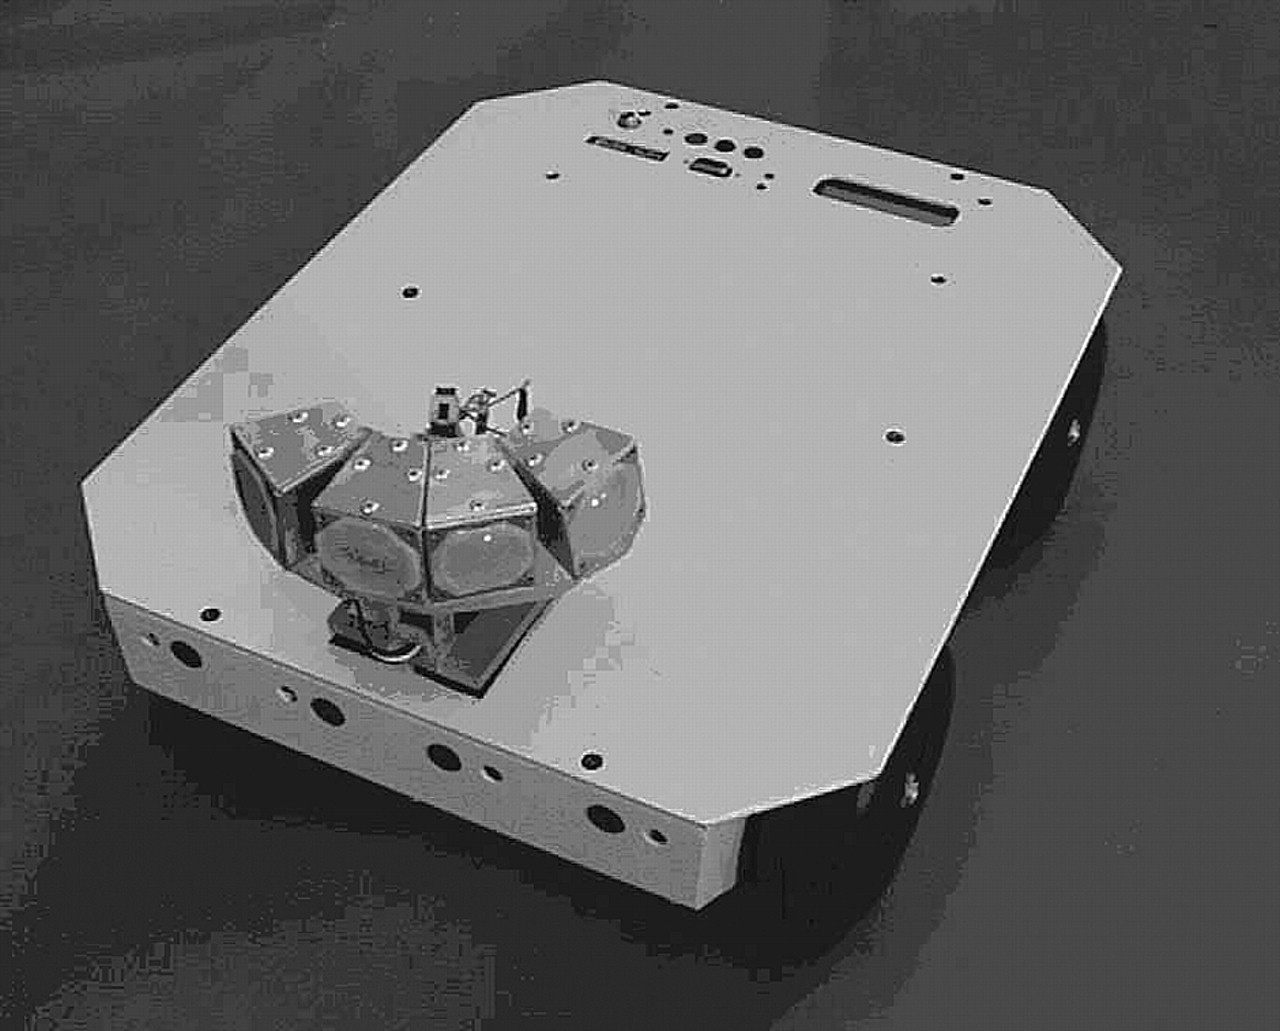
\includegraphics[width=4.5cm]{labo1}
		 \caption{Labo-1}
		 \label{fig:Labo1}
	\end{subfigure}
	\begin{subfigure}[b]{0.3\textwidth}
		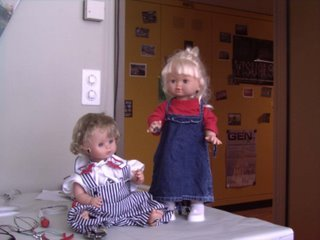
\includegraphics[width=4.8cm]{robota}
		 \caption{Robota}
		 \label{fig:Robota}
	\end{subfigure}
	\begin{subfigure}[b]{0.4\textwidth}
		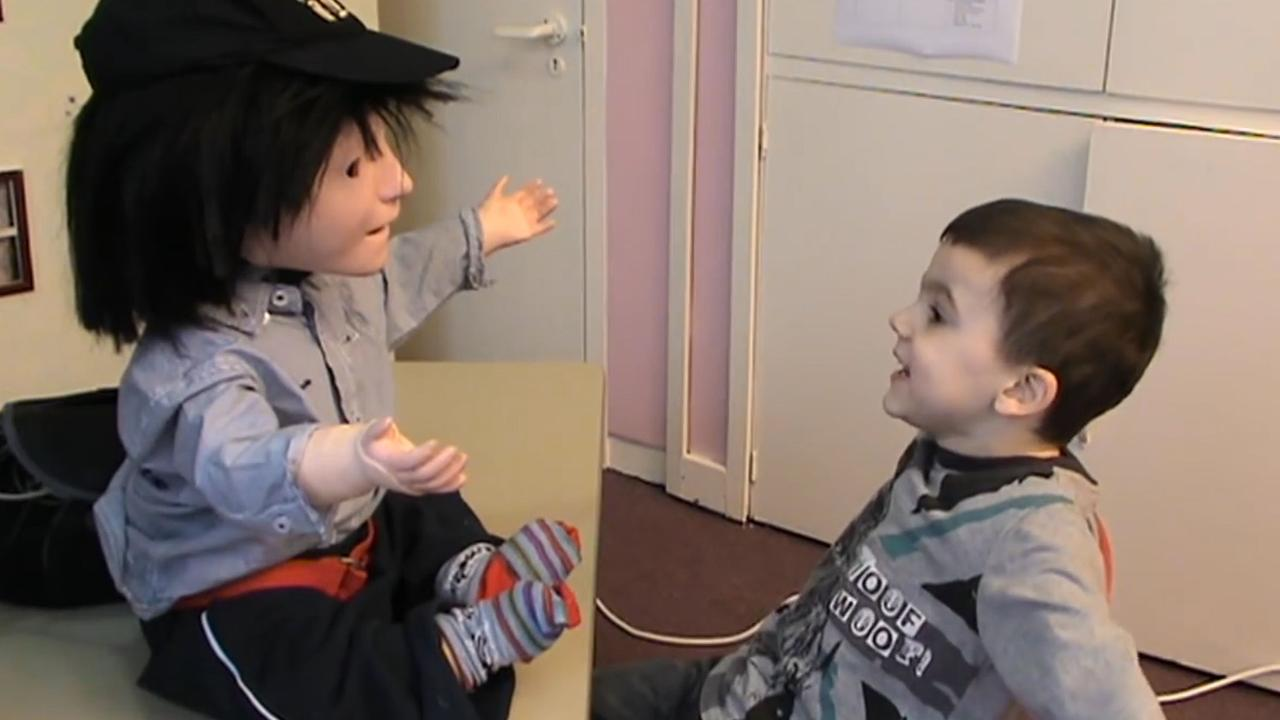
\includegraphics[width=6cm]{kaspar}
		 \caption{Kaspar}
		 \label{fig:Kaspar}
	\end{subfigure}
	\rule{35em}{0.5pt}
	\caption{Robots developed by Aurora Project}
	\label{fig:AuroraProjRobots}
\end{figure}

\subsection{Labo-1}
Labo-1 was the first robot developed by Aurora project\cite{werry1999applying}.It is a robust and \textit{mobile} flat-topped robot with 4 wheels, 8 infrared sensors, 1 heat sensor and, from the second version, 1 speech synthesizer. Thanks to its sensors, it is able to produce short spoken phrases using a neutral intonation and follow or escape from children avoiding obstacles. Its robustness and weight makes Labo-1 hard to pick up or damage from children. 
Trials done with four boys, aged between 8 and 12 years old, in order to improve \textbf{triadic interaction} and \textbf{turn-taking}.In a room with children, robot and therapist, the child was engaged in games that alternate the robot following turn to the go around turn. Children interacted with the robot without fear: some of them tried to clear obstacles from robot's path, one child smiled to the therapist for share his excitement and others tried to understand the robot's behavior observing its reactions to their continuous actions.
\subsection{Robota}
In 1998 the Aurora Project developed Robota\cite{billard1998experiments}, a doll-shaped humanoid robot. Its has motors that make arms, legs and eyes movable, it can speak thanks to his speech synthesizer, and can also understand lots key-words. Its camera processes the video, making Robota able to understand children movements and where they are looking to. When a children looks the robot, it starts to reply the movements performed by the children. This result as an improve in \textbf{imitation} and \textbf{eye-contact} behaviors. 
Robota was later\cite{billard2003robota} incorporated with a set of games focused on improve logic, coordination, and intellectual skills. This games are: dress the robot in the correct order, draw movements or positions in a PC or tablet that will be replayed by the robot, and interact(touching o performing movements) with the robot for answer to additions questions. Despite Robota seems to not intimidate children and during the studies were observed clear sign of enjoyment and social interaction, such as smiling and say goodbye, any case of spontaneous interaction occurred: it was always initiated by the teacher. Subsequent studies compared self-initiated interaction based on appearance, making trials with classic Robota and a plain version without eyes, hairs and plain dress. That study concludes that \textbf{children prefer to interact with a plain robot over a human-like robot}\cite{billard2007building}.

\subsection{Kaspar}
KASPAR is a minimally expressive \textbf{child-sized} humanoid robot designed for social interaction. In order to make it more attractive for ASD children, Kaspar has \textbf{simplified face} than an human(see appearance in \ref{designF}). It can show facial expressions, move his arms, hands, torso, head\cite{huijnen2016matching}, and speak using pre-recorded traces. It is used in \textbf{semi-autonomous manner}: the expert controls some Kaspar functionalities while other action are triggered from the robot sensors .
Children are encouraged in tactile exploration on Kaspar body and to repeat his facial expression, encouraging \textbf{eye-gaze} and increasing \textbf{emotion recognition} and body awareness with \textbf{turn-taking} \textbf{imitative} games. Another KASPAR’s purpose is to promote collaborative play with other children and adults, improving \textbf{triadic interaction}, and \textbf{joint attention}. 

The researchers conducted a study\cite{dautenhahn2009kaspar} in order to investigate how this robot could mediate the interaction between children with autism
and other people. During the interactions with KASPAR, children did not demonstrate aggressive behaviors towards the robot, they touched and gazed to its facial expressions in detail and also interacted with the present adult and social peers. So, it was possible to observe that KASPAR helped all the participants \textbf{to generalize their behavior} with the robot to others.

\section{Tito}
Tito\cite{duquette2008exploring} is a \textbf{mobile robot} with anthropomorphic shape. It has human stylized features such as movable arms, head and feet, despite it uses wheels for motion. Its face is composed by two eyes, a nose, and movable mouth. In one of the eyes, it has a camera able to measure eye gaze toward him. It uses pre-recorded messages for communication and it is controlled by wireless. Different parts of
Tito’s body can also be illuminated, and it is able to sense if it is being shaken or if it has flipped over.
\begin{figure}[h]
	\centering
	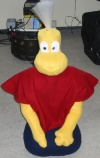
\includegraphics[width=0.4\textwidth]{tito}
	\caption{Tito}
	\label{fig:Keepon}
\end{figure}
Robots in general are more predictable and
less complex in their interacting modalities compared with a human and this robot has been created in order to analyze how effective are robots for ASD therapy compared with humans. A group of four children was split in two groups of two children each. The first group interacted with a robot mediator, the other one with a human mediator. In both cases children were engaged in three levels of imitation exercises: facial expressions, body movements, and familiar actions with or without objects. In both group, when the children imitated correctly, the mediator gave a sensory reward smiling, raising both its arms and saying 'Happy!'. The results showed that participants paired with Tito demonstrated more shared focused attention, visual contact, facial expression imitation and eye gaze directed toward the robot than ones paired with a human mediator. However, the children paired with the human mediator demonstrated, compared to the others, more evident increase on the imitation of words, gestures and body movements towards the other person in the room. 
In conclusion, the study showed that sensory properties of the robot (e.g. movements, colors, lights) managed to keep children interested in it but children paired with the human revealed higher results on imitation of body movements and of familiar actions. The authors hypothesized it was due to the restricted movement capabilities of the robot that did not allow children to understand their communicative intent.

\section{Keepon}
Hideki Kozima and his research group of Kyoto National Institute of Information and Communications Technology, developed interesting studies in the field of social robots for autism therapy\cite{kozima2009keepon}. Previously they built Infanoid, a upper-torso humanoid robot able to show facial expressions and other gestures. Researchers observed that the robot highly mechanistic appearance and its excessive expression of information caused attention dispersion and led to anxiety. Therefore, the researchers developed Keepon that, unlike Infanoid, has a minimal design that makes children feel more comfortable.
\begin{figure}[h]
	\centering
	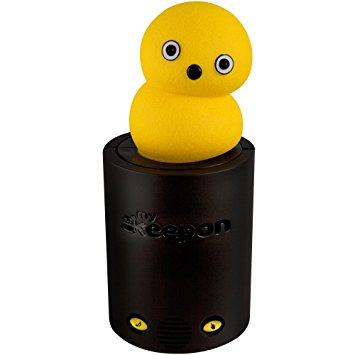
\includegraphics[width=0.4\textwidth]{keepon}
	\caption{Keepon}
	\label{fig:Keepon}
\end{figure}
Keepon is an anthropomorphic robot with a yellow snowman-like body, it is 12 cm tall and it is composed by tho parts: the head and the belly. The head has two eyes and a nose. Thanks to four DC motors, the silicon rubber material it is made, and small gimbals and wires installed in the belly, it is possible to manipulate Keepon's body, like a marionette.
Keepon can be autonomous or remote controlled, and it can orienting its face to a certain target and express its emotional states whenever the child makes any verbal or physical social interaction. It also interact coming up with rhythmic games, in form of structured music and dance sessions or with repetitive \textbf{turn-taking} and \textbf{imitation} behavior. Body movements are preprogrammed and it can exhibit excitement, pleasure and fear \textbf{emotions}, or simply dance.
Researches analyzed how the minimal design of Keepon could help children to understand social information and motivate them to share interests and feelings with others. Trials demonstrated that children spontaneously approached and started “tasting” Keepon's texture and motion, entering gradually into a complete social interaction with the robot. Thanks to simple and comprehensible ways used by the robot for exhibit its attention and emotions, children could understand the social meaning of the robot’s actions without becoming bored or overwhelmed. \textbf{Triadic interaction} and \textbf{joint attention} with peers and adult was also improved for some children: one children stops another while he was beating the robot; others shared joy or surprise to adults while they were interacting with the robot.
The research conclusion was that simple robots with  minimal and comprehensible expressiveness make easier understanding and extracting socially meaningful information for ASD children, encouraging so the expression of emotional states like surprise, pleasure or frustration.
\section{Paro}
PARO is an autonomous robotic seal equipped with sensors and actuators and computational intelligence that enables it to simulate the sounds and movements of a real baby harp seal. It has five kinds of sensors: tactile, light, audition, temperature, and posture sensors, with which it can perceive people and its environment. With the light sensor, PARO can recognize light and dark. He feels being stroked and beaten by tactile sensor, or being held by the posture sensor. PARO can also recognize the direction of voice and words such as its name, greetings, and praise with its audio sensor. It can also learn to behave in a way that the user prefers, changing the probability to do an action based on previous reaction(an hit or a pat) to that action. It can also responds to verbal question, moving its head, legs and making sounds. 
It is being used with great success in dementia care in Japan and Europe as a robot companion with the purpose of increasing quality of life and reduce stress and anxiety and to provide a therapeutic tool for specific individual interventions. Research suggests that PARO can be used as a facilitator of social communication for children with autism as well (Roberts \& Shore, 2013).
Researchers\cite{bertel2013peers} also conducted a three month case study on the use of PARO, at a school for children with autism, in order to study long-term interactions in real-world educational settings. The robot is used in order to motivate\textbf{ bodily or verbal attention}, involving children to touch it and to verbalize their thoughts; \textbf{create joint attention} with peers, asking children to touch the robot together touching eventually each other; \textbf{motivate social attention}, putting Paro in the center of a group of children and singing all together; and to \textbf{redirect attention}, asking children to help him in some activities.



\section{Nao \& Zeno}
Nao, developed by ,and Zeno, developed by, , are both \textbf{small-size humanoid} robots used for \textbf{imitative} and \textbf{turn taking} games. Therapy sessions are done with the robot placed on a table and the children sit on a chair in front of that. These robot can imitate children movements or engage them to imitate their movements, giving a positive sensory reward when the imitation is well done, or trying to motivate more or help the children if he is not able to imitate the movement. Zeno is used also to ask children to guess its mood. These robots are provided with a software for easy program the robot's behavior, and this makes them very customizable and this has permitted to use them for a lot of different studies. The setting of the interaction, unfortunately, results poor for autistic children: a therapist that controls the children does not touch the robot is needed, being the robot expensive and quite delicate. Another negative point are their rigid and jerky movements that furthermore need to be monitored because the robot can fall from the table. 
\section{Previous Teo}
Teo is an emotional, huggable, mobile and configurable robot developed by Politectico di Milano. Thanks to three omnidirectional wheels, its movement is holonomic, allowing it to freely move in any direction. Hidden on its body, Teo has a set of force sensing resistors that make it able to detect and distinguish hugs, caresses and punches. It is also equipped by a set of big mechanical buttons located on the head that can be personalized and permit children to express choices in response to different situation. A set of colored light, hidden in the body, are used to strengthen interaction and express emotions. An external depth sensor(kinect) can sense the motion of children making possible to display on a screen a virtual reality that encourages children to have a full-body interaction with the robot. 
Teo's cartoon-like with human simplified characteristics design stimulate ASD children to explore the interaction with it without any fear. One of the most important Teo's characteristic is personalization: sets of different mouths and eyes can be placed on the robot, creating a large number of different expression, or can be completely taken out, removing any human trait and making Teo more like an object than a person. Also mechanical buttons can be personalized, based on the ongoing activity or game, by colored tags or iconic images.
Teo can be remotely controlled, but it has also autonomous behaviors activated when sensors detect an interaction or during games.
\begin{figure}[h]
	\centering
	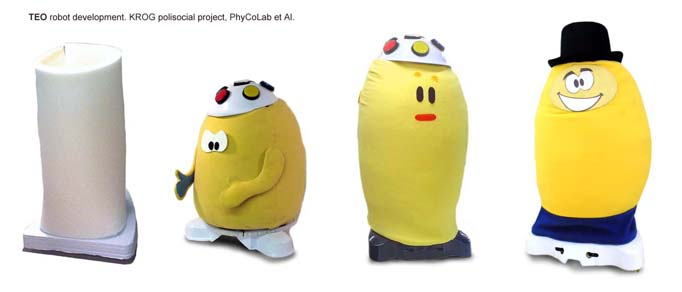
\includegraphics[width=0.9\textwidth]{prevTeo}
	\caption{Teo's shape history}
	\label{fig:prevTeo}
\end{figure}
Teo has been used in two exploratory studies. The first study involved 19 children aged between 6 and 12 years old that were split in two groups: one group, composed by children with most severe cognitive deficits, played alone, while children whose socialization problems were more severe than cognitive deficits, played with a peer. Three sessions were held weekly, the third was a group session, where children interact with Teo and all their classmates. Results highlights the importance to make more than one session with the robot: in both groups has been noticed an increase of positive behavior from the first session to the second. That increase, noticed in communication's skills, self-expression ability, attention loss frequency and interaction, was stronger in paired session, suggesting that group sessions are more effectively than alone ones. 
The second study involved 5 low functioning autistic subjects playing alone under a therapist's supervision for 10 weekly held sessions. In this study patients were engaged to answer to color-related questions made by Teo, touching the right button. A comparison between the number of right answers obtained 'with' and 'without' Teo emphasizes a wide difference, demonstrating the robot effectiveness.
